\documentclass[12pt]{article}
\usepackage{fullpage}
\usepackage{listings}
\usepackage{hyperref}
\usepackage{amsmath}
\usepackage{multirow}
\usepackage{array}
\usepackage{boldline}
\usepackage{hyperref}
\usepackage{graphicx}


\title{SpMV Calculation using GPU(Apple Metal) and CPU(OpenMP)}
\author{Zehong Wang}
\date{2023-05-01}

\lstset{
    frame=single,
    breaklines=true,
    basicstyle=\ttfamily,
    language=bash,
}

\begin{document}

\maketitle

\section{Introduction}
This project implements a Sparse Matrix-Vector Multiplication (SpMV) calculator using CSR and COO formats and optimizations on both CPU and GPU. The program loads a sparse matrix and a vector from a file, and calculates the matrix-vector product.

\begin{itemize}
    \item The GPU part is implemented using \textbf{Apple Metal Shading Language}
    \item The CPU part is implemented using \textbf{OpenMP}
\end{itemize}

\section{Hardware Requirement}
This program can only run on \textbf{Apple Chip Laptop}, such as M1, M1 Pro, M1 Max, M2, M2 Pro, M2 Max.

\section{Environment Setup}
\begin{lstlisting}
# Install llvm version of clang to support OpenMP
brew install llvm
# Install OpenMP
brew install libomp
# Install GSL
brew install gsl
# Install cmake
brew install cmake
# Install XCode Command Line Tools to support Metal Compiler
xcode-select --install
\end{lstlisting}

\section{Runnning Command}
The program \textbf{error tips are very friendly}, so you can just run the program and see the tips.

\begin{lstlisting}
cmake .
make && make kernel
./spmv xxx.mtx
\end{lstlisting}

\section{File Structure}

\subsection{spmv.metal}
This is the Metal kernel using Metal Shading Language. It provides three kernel functions to perform Sparse Matrix-Vector Multiplication (SpMV) using different formats and optimizations on GPU.

\begin{itemize}
    \item \textbf{spmv\_csr} \\
    This kernel function calculates the SpMV product using the CSR format. It takes in row pointers, column indices, values, input vector `x`, and an output vector `result`. The kernel processes each row of the sparse matrix in parallel.

    \item \textbf{spmv\_coo} \\
    Optimization 1 for `spmv\_csr`. This kernel function calculates the SpMV product using the COO format. It processes the non-zero elements of the sparse matrix in parallel. It takes row indices, column indices, values, input vector `x`, and an output vector `result` (\textbf{with atomic float type}).

    \item \textbf{spmv\_csr\_loop\_unrolling} \\
    Optimization 2 for `spmv\_csr`. This kernel function applies loop unrolling optimization. The loop unrolling is performed with a step of 4 to potentially improve performance.
\end{itemize}

\subsection{spmv\_calculator.h / spmv\_calculator.cpp}
The \textbf{SpmvCalculator} is responsible for performing SpMV calculations using different approaches:

\begin{itemize}
    \item GPU with CSR format
    \item GPU with CSR format and loop unrolling optimization
    \item GPU with COO format
    \item CPU with serial processing
    \item CPU with OpenMP parallel processing
\end{itemize}

It also provides a method for verifying the results.

\subsection{logger.h / logger.cpp}
The \textbf{Logger} provides static methods for logging messages of various levels: `info`, `error`, `debug`, and `warn`. It also includes a method, `time`, for measuring and logging the time taken by specific operations.

\section{Research and Design}
\begin{itemize}
    \item The Apple GPU with Metal Shading Language (MSL) can run up to \textbf{1024} threads. Technically, it can achieve a \textbf{1000x} speedup, confirmed by running all the computations inside a single kernel; the code logic was omitted.
    \item GPU MSL kernel optimization is not as efficient as CPU optimization, such as shading overhead and kernel compiler optimization. Therefore, it experiences performance loss.
    \item The basic algorithm uses CSR and assigns each row to a thread, which then serially loops through the non-zero values in the row to compute the final results.
    \item Optimization 1: Employ COO format instead of CSR, distributing all non-zero values to each GPU thread and atomically summing the results. While this algorithm should outperform the CSR format, atomic reduction overhead and memory cache issues prevent significant improvement.
    \item Optimization 2: Since Metal GPU compiler optimization is less mature than C++, loop unrolling can lead to significant speedup due to SIMD optimization.
\end{itemize}

\section{Performance}

\subsection{Conclusion}
\begin{itemize}
    \item CPU OpenMP with 4 threads achieves a \textbf{4x} speedup compared to the CPU Serial Version (\textbf{TEST-1} vs \textbf{TEST-2}, \textbf{TEST-6} vs \textbf{TEST-7}).
    \item GPU COO runs \textbf{slightly faster} than GPU CSR (\textbf{TEST-3} vs \textbf{TEST-5}, \textbf{TEST-8} vs \textbf{TEST-10}).
    \item GPU CSR with loop unrolling optimization achieves a \textbf{2x} speedup (\textbf{TEST-3} vs \textbf{TEST-4}, \textbf{TEST-8} vs \textbf{TEST-9}).
    \item CPU Serial and OpenMP versions attain a \textbf{6x} speedup with `-O3` compiler optimization (\textbf{TEST-1} vs \textbf{TEST-6}, \textbf{TEST-2} vs \textbf{TEST-7}).
    \item GPU CSR provides a \textbf{25x} speedup compared to the CPU Serial without compiler optimization and a \textbf{4x} speedup compared to CPU Serial with `-O3` optimization (\textbf{TEST-1} vs \textbf{TEST-4}, \textbf{TEST-6} vs \textbf{TEST-9}).
    \item Comparing the best versions, the GPU still runs faster than the CPU (\textbf{TEST-7} vs \textbf{TEST-9}).
\end{itemize}

\subsection{Running Results}
\begin{itemize}
    \item Results Table
    
    \begin{minipage}{\linewidth}
    \centering
    \begin{tabular}{|c!{\vrule width 1pt}c|l|c|}
    \hlineB{2}
    \multicolumn{1}{|c!{\vrule width 1pt}}{CPU Compiler} & Test Number & Test Item                           & Time (ms) \\
    \multicolumn{1}{|c!{\vrule width 1pt}}{Optimization} &             &                                     &           \\
    \hline
    \multirow{5}{*}{[-O0]}    & 1           & CPU Serial Version                  & 7467      \\
    \cline{2-4}
                              & 2           & CPU OpenMP Version                  & 1858      \\
    \cline{2-4}
                              & 3           & GPU CSR Version                     & 625       \\
    \cline{2-4}
                              & 4           & GPU CSR with Loop Unrolling Version & 297       \\
    \cline{2-4}
                              & 5           & GPU COO Version                     & 606       \\
    \hline
    \multirow{5}{*}{[-O3]}    & 6           & CPU Serial Version                  & 1152      \\
    \cline{2-4}
                              & 7           & CPU OpenMP Version                  & 398       \\
    \cline{2-4}
                              & 8           & GPU CSR Version                     & 627       \\
    \cline{2-4}
                              & 9           & GPU CSR with Loop Unrolling Version & 294       \\
    \cline{2-4}
                              & 10          & GPU COO Version                     & 578       \\
    \hlineB{2}
    \end{tabular}
    \end{minipage}
\end{itemize}

\begin{itemize}
    \item CPU applies [-O0]
    
    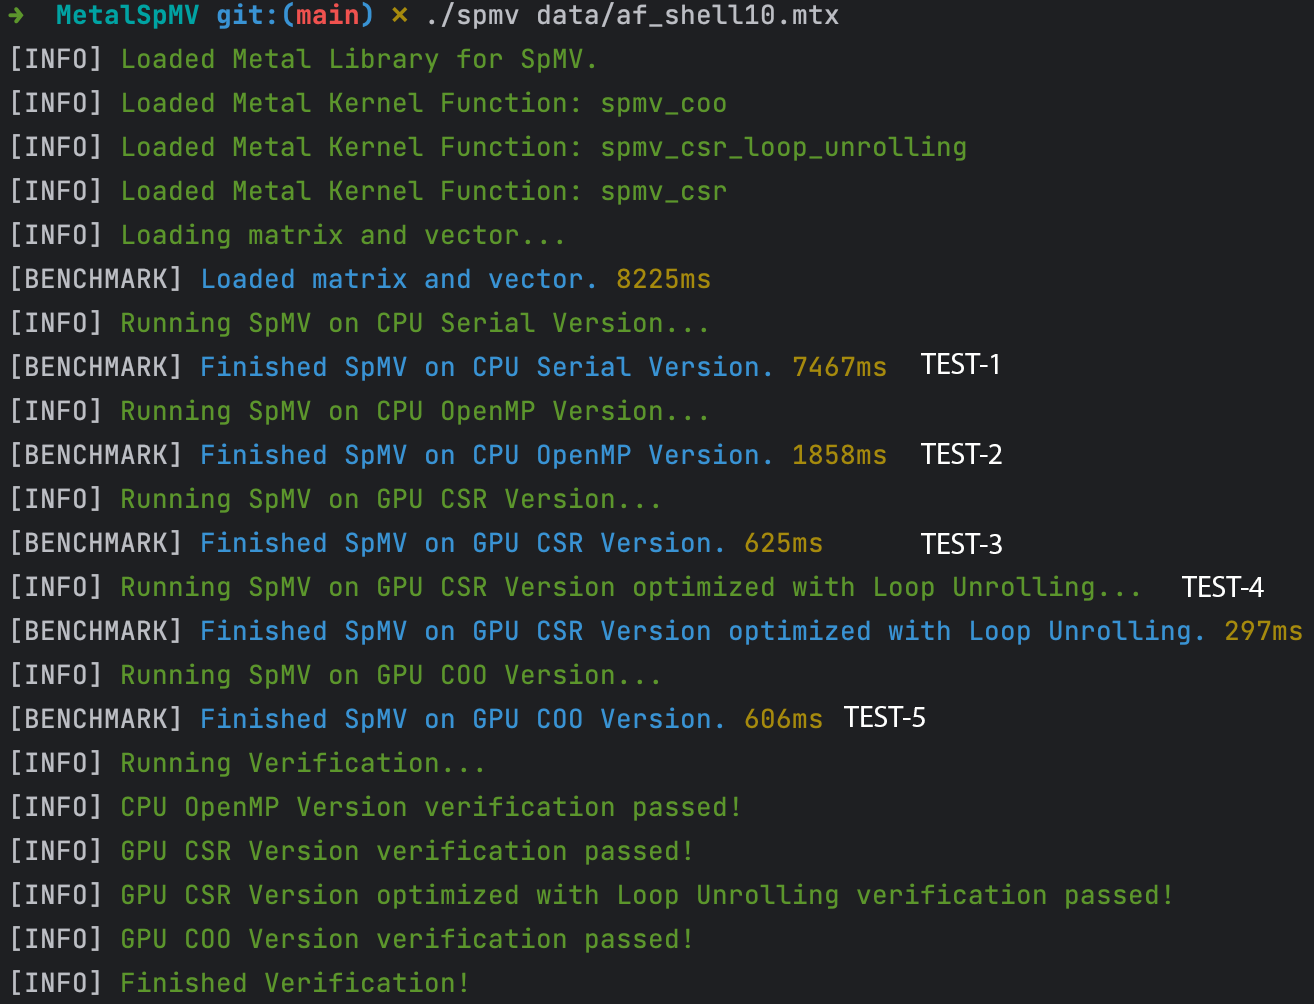
\includegraphics[width=0.75\textwidth]{./images/CPU_O0.png}
    
    \item C++ applies [-O3]
    
    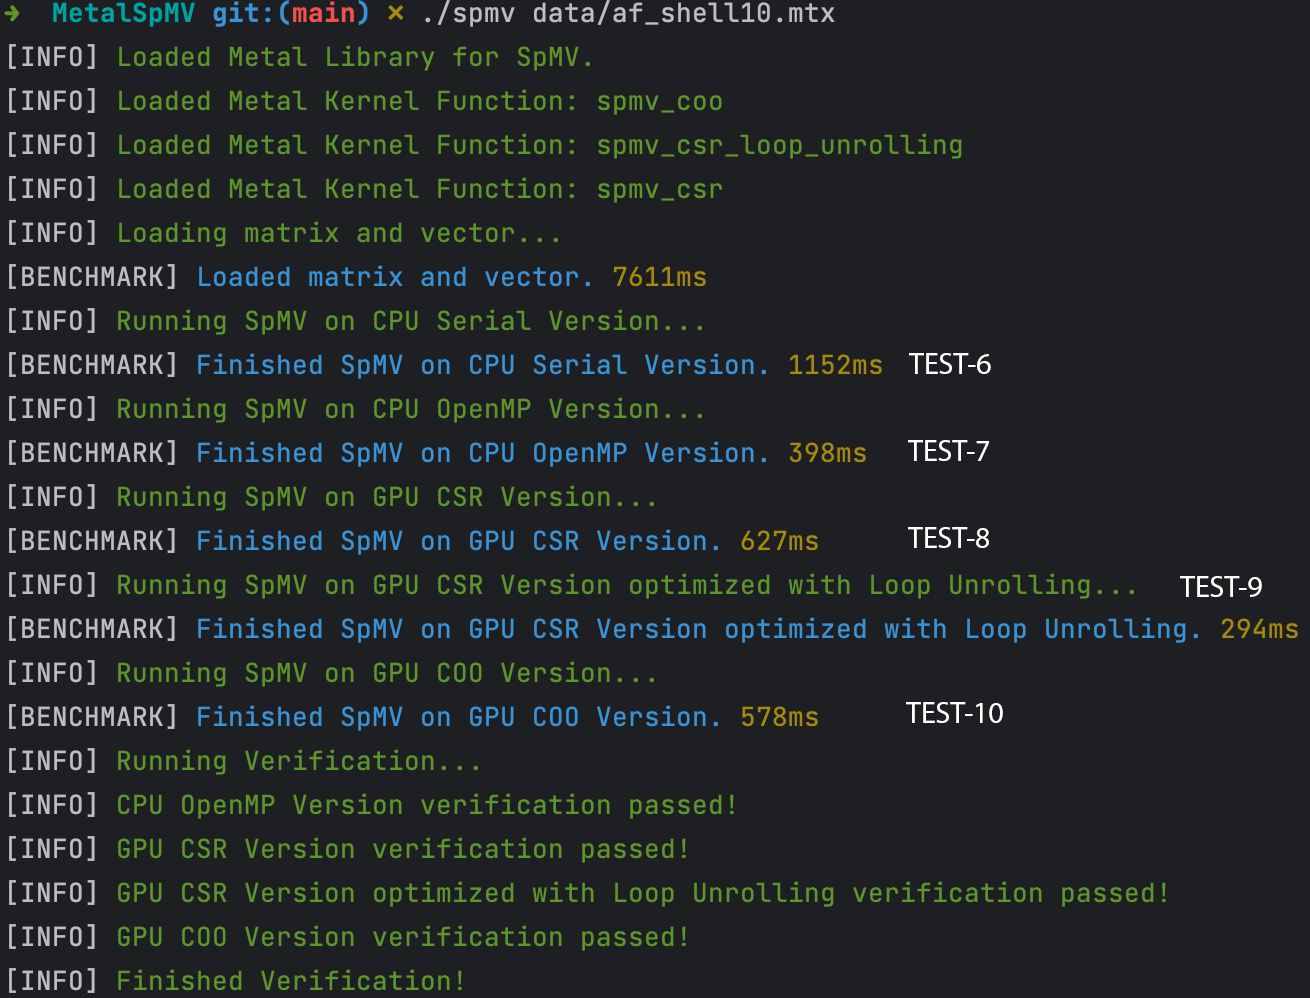
\includegraphics[width=0.75\textwidth]{./images/CPU_O3.png}
    \end{itemize}

\section{Available Matrix Collection}

\begin{itemize}
\item \href{https://suitesparse-collection-website.herokuapp.com/RB/Schenk/nlpkkt80.tar.gz}{nlpkkt80}
\item \href{https://suitesparse-collection-website.herokuapp.com/MM/Schenk_AFE/af_shell10.tar.gz}{af\_shell10}
\item \href{https://suitesparse-collection-website.herokuapp.com/MM/Janna/StocF-1465.tar.gz}{StocF-1465}
\end{itemize}

\end{document}
